

\documentclass[10pt, conference, compsocconf]{IEEEtran}

\ifCLASSINFOpdf

\else

\fi

\usepackage{hyperref}
\usepackage{amsmath}
\usepackage{amssymb}
\usepackage{hhline} % easy to manage table borders
\usepackage{colortbl} % colored cells in tables
\usepackage{multirow}
\usepackage{enumerate}
\usepackage{slashbox} % cell with slash inside
\usepackage{makeidx}  % allows index generation
\usepackage[utf8]{inputenc}
\usepackage{graphicx}

\newtheorem{definition}{Definition}
\newtheorem{example}{Example}

\def\sectionautorefname{Section}
\def\subsectionautorefname{Section}


% correct bad hyphenation here
\hyphenation{op-tical net-works semi-conduc-tor}


\begin{document}

% paper title
% can use linebreaks \\ within to get better formatting as desired
\title{Pharmer -- Semantic Authoring of Medical Prescriptions}
%\title{Pharmer: A platform for health care providers to use linked open data in e-prescriptions}


% author names and affiliations
% use a multiple column layout for up to two different
% affiliations

\author{\IEEEauthorblockN{Ali Khalili}
\IEEEauthorblockA{Faculty of Computer Science\\
University of Leipzig\\
Leipzig, Germany\\
khalili@informatik.uni-leipzig.de}
\and
\IEEEauthorblockN{Bita Sedaghati}
\IEEEauthorblockA{Institute of Pharmacy\\
University of Leipzig\\
Leipzig, Germany\\
bita.sedaghati@uni-leipzig.de}
}


% make the title area
\maketitle

\begin{abstract}
The abstract goes here. DO NOT USE SPECIAL CHARACTERS, SYMBOLS, OR MATH IN YOUR TITLE OR ABSTRACT.

\end{abstract}

\begin{IEEEkeywords}
component; formatting; style; styling;

\end{IEEEkeywords}


\IEEEpeerreviewmaketitle



\section{Introduction}
This is a test \cite{Khalili2012}.

While even nowadays traditional paper prescriptions are commonly used, electronic prescriptions offer several advantages.
As reported in \cite{} medication errors are the most common type of medical error in health care.
In an E-prescription system, prescriber electronically sends an accurate, error-free and understandable prescription directly to a pharmacy from the point-of-care.
Improved confidentiality and security of health information, better clarity and communication among health care providers as well as rapid information exchange are part of arguments for spreading this system.
Reduction in medication error and decline in adverse drug events are more highlighted consequences of E-prescribing.

During the recent years, the adoption of E-prescriptions has been spreading rapidly.
To illustrate, the Australian government started launching of e-prescription from 1 March 2007.
Using this system, the e-providers who effectively market themselves on the web will have a distinct advantage\cite{Ravichandran}.
A system called epSOS perform the use of E-prescriptions all around Europe, is currently passing the extensive practical testing phase.
It contains patient summery and E-Prescription Service which allows access to the cross-border eHealth services when seeking healthcare in participating epSOS pilot countries, as tourists, business travellers, commuters or exchange students.
The E-Prescribing Incentive Program is performed in US as a reporting program that uses a combination of incentive payments and payment adjustments to encourage electronic prescribing by eligible professionals.

One of the most important advantages of E-prescribing is that the connection of physician, pharmacist, patient and pharmaceutical researchers and statision.
Once the E-prescription is written by a physician, pharmacist has also access to the prescription.
while the physician is aware, pharmacist can comment on the prescription content.
The online system is also available for patients who can inquire about any necessary information.
health care providers can follow up the patient's treatment fate.
The data base of the patients profile in subject of many statistics researches.
Besides, researchers are able to conveniently follow the drug in the clinical trial phase.



\section{Semantic Content Authoring}
\label{sec:sca}

\section{E-Prescriptions}
E-health has evolved and emerged recently in many forms.
E-prescription is one of these forms and defined as a computer-generated prescription utilized by healthcare providers.
E-prescribing as it is commonly called, is the use of an automated data entry system to generate a prescription that is then transmitted through a special network to the pharmacy in such a way that the data goes directly into the pharmacy’s computer system.
It plays an important role in improving the quality of patient care.
For the prescriber, e-prescribing happens when a physician uses a computer or hand held device with software that allows him or her to—with a patient’s consent—electronically access information regarding a patient’s drug benefit coverage and medication history; electronically transmit the prescription to the patient’s choice of pharmacy; and, when the patient runs out of refills, his or her pharmacist can also electronically send a renewal request to the physician’s office for approval.

There are challenges that are solved by E-prescription systems.
Once writing a prescription it is very critical to consider drug interactions.
Drug interactions are divided to three categories namely \emph{food-drug}, \emph{drug-drug} and \emph{drug-plant} interactions.
Coadministration can either be synergistic or antagonistic which respectively increase or decrease the drugs effect.
The interactions may sometimes lead to change in the drug effect.
By applying E-prescription system, all types of drug interactions are prevented and the probability of errors in prescriptions are reduced to a great extend.
A E-prescription simply contains drug information and precautions which are necessary to be considered from patient's side.

Through electronic prescribing, all health care stakeholders including providers, patients, pharmacies, and payors benefits such as:
Payors/insurances: efficiency, prescription compliance and prevention of Adverse drug reactions.
Patients: Increased safety, efficiency and compliance, lowered co-pays
Providers: Increased efficiency, improved care, patient satisfaction and potential short and long-term incentives
Pharmacies: Increased efficiency, improved care, improved patient satisfaction

E-prescribing involves far more than an electronic connection. In order to see an increase in both quality and efficiency that can be attributed to e-prescribing, the system must be capable of performing key functions related to:
Medication selection/decision support capabilities (e.g., diagnosis-based medication menus, evidence based information, drug interaction checking, safety-alerts, formulary checking, prescription renewal, and dosage calculation)
Patient-specific information capabilities (e.g., current patient medication list, access to patient historical data, patient identification)
System integration capabilities (e.g., connection with various databases, connection with pharmacy and pharmacy benefit manager systems)
Educational capabilities (e.g., patient education, provider feedback)

The journey of an e-script begins when the patient and physician review history and discuss the current issue and treatment options. The patient’s up-to-date formulary and medication history is then presented to the provider at the point-of-care.
The physician then reviews clinical alerts, formulary, reference, prescription history and eligibility with the patient and selects therapy and verifies the patient’s preferred pharmacy.
Once the prescription is finalized, the e-script is generated and the physician routs it to the patient’s pharmacy of choice. The pharmacist fills the prescription and sends a fill notification to the physician.
The two-way connectivity provides for the transmission of new prescriptions, refill authorizations, and denials and change requests between the pharmacy and the provider’s office.

It is also evident by using the E-prescription, follow up of patient individuals is convenient.The next part of procedure occurs during the medication therapy and afterwards. The patient is supposed to report about his/her condition by returning to a physician or online contact.
The health care providers can access to the patient's profile and the transfer of these data can appropriately be done.
Besides, the data of medicines consumption and the connection between diagnosed disease and the treatment regimen is recorded.
Furthermore, patient's fate after the medication duration can be followed up by physicians and pharmacists.
The E-prescription information is  of crucial importance as an  informative source for researchers.
Many researchers investigate the aforementioned statistical data and combine them with the information received from the medicine producers (e.g. to compare the special drug consumption different  individual age ranges).


Another challenge points 

 and needs to be more carefully investigated by health care providers. 



\section{Semantic Authoring of Medical Prescriptions}

\section{Pharmer}
In \autoref{fig:lod}, you can see..
We discussed sth in \autoref{sec:sca}.

\subsection{Architecture}

\begin{figure}[tb]
	\centering
		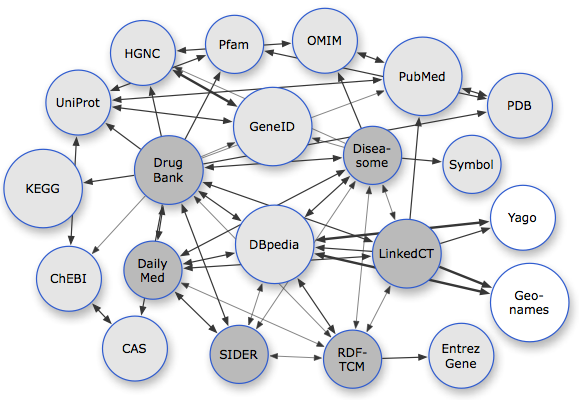
\includegraphics[width=1.0\columnwidth]{images/lod_cloud.png}
	\caption{Available datasets related to pharmaceutical research.}
	\label{fig:lod}
\end{figure}


\section{Conclusion}
The conclusion goes here. this is more of the conclusion

% conference papers do not normally have an appendix


% use section* for acknowledgement
\section*{Acknowledgment}


The authors would like to thank...
more thanks here

\bibliographystyle{IEEEtran}
% argument is your BibTeX string definitions and bibliography database(s)
\bibliography{refs}





% that's all folks
\end{document}


